\subsection{Diagramme de classes de conception préliminaire}
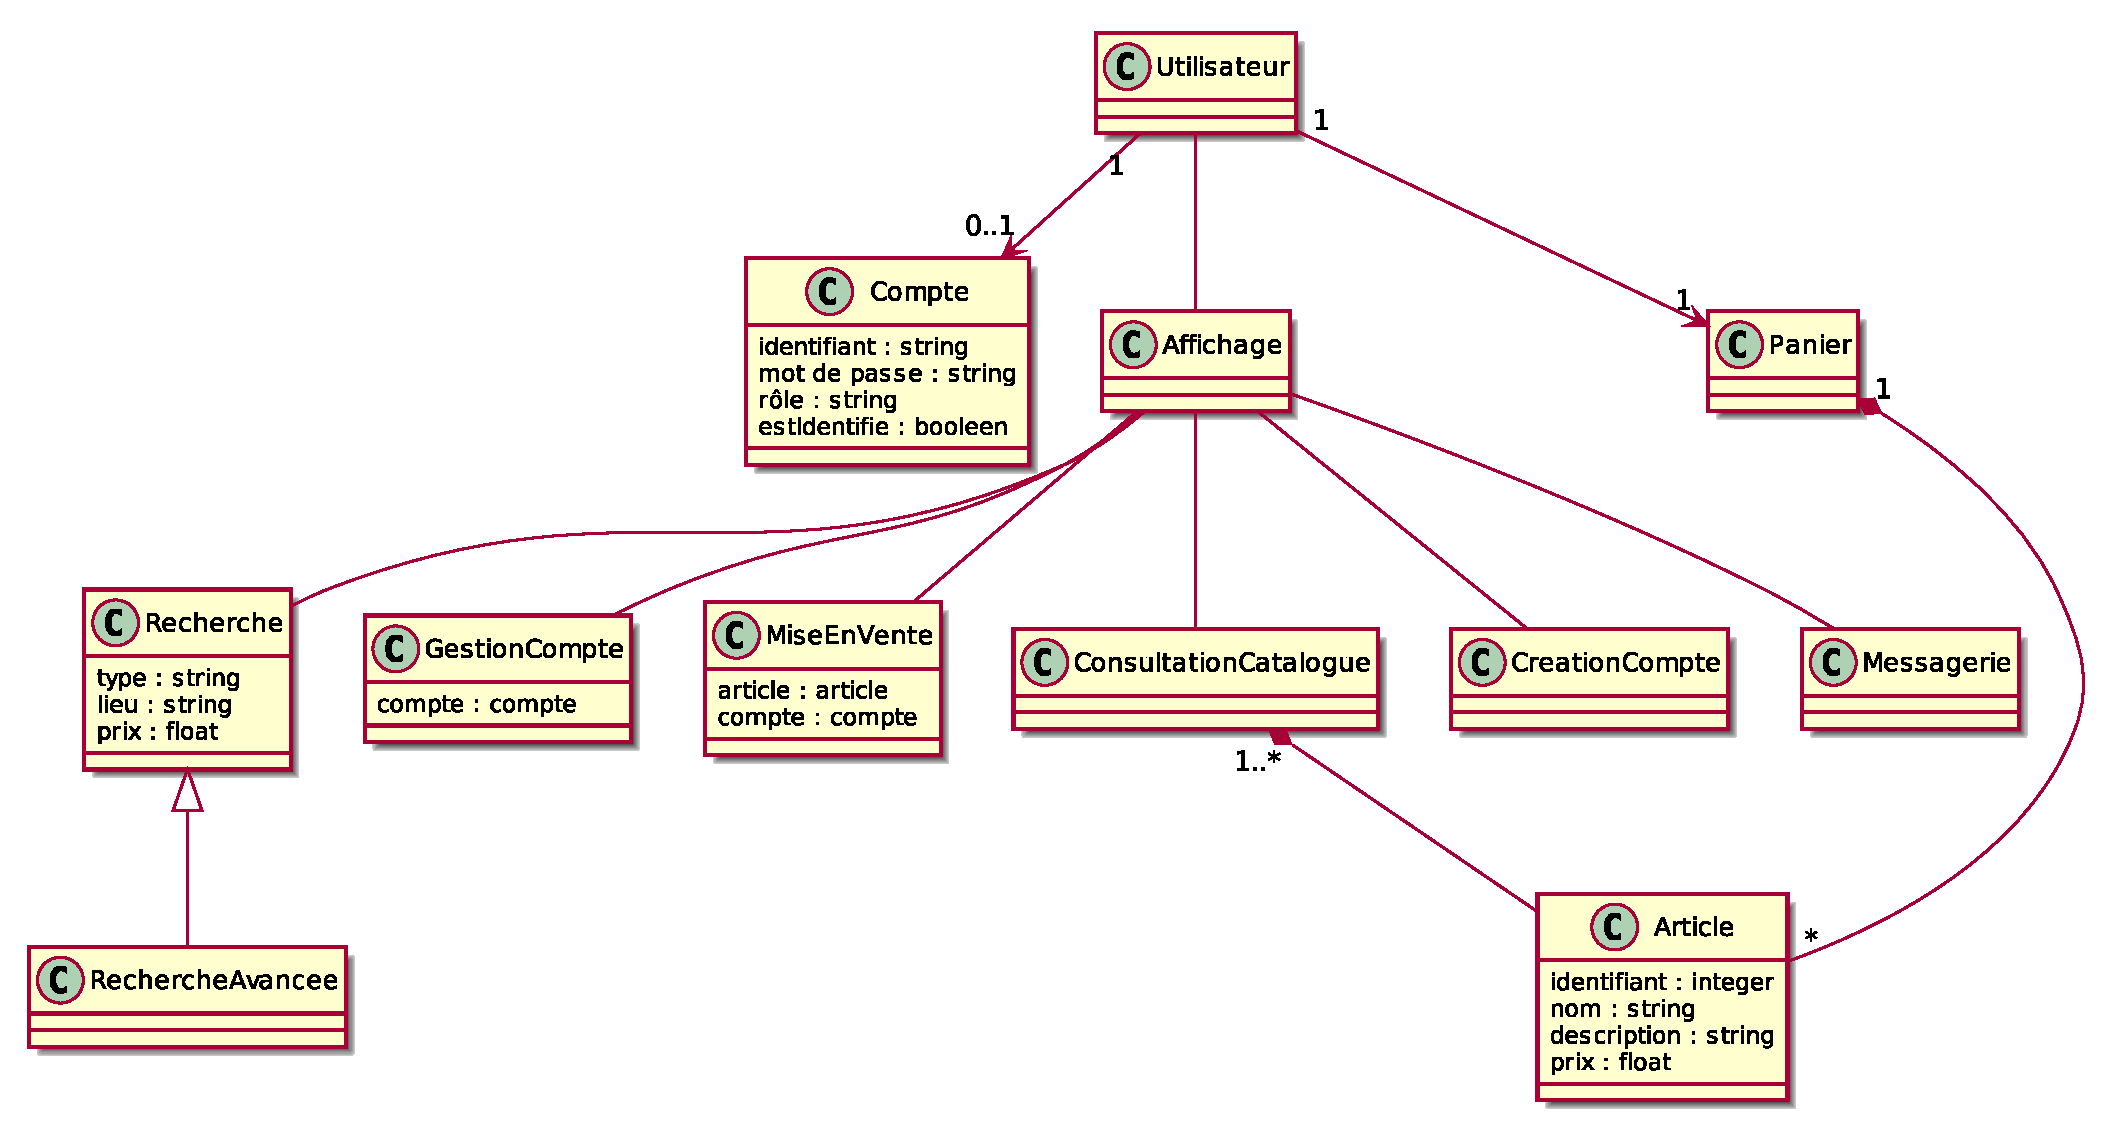
\includegraphics[width=17cm]{Images/DCCP} \\

\newpage
\subsection{Diagrammes de séquence}

\subsubsection{Création d'un compte}
Un visiteur peut créer un compte sur le site en renseignant ses informations et un mot de passe associé.\\
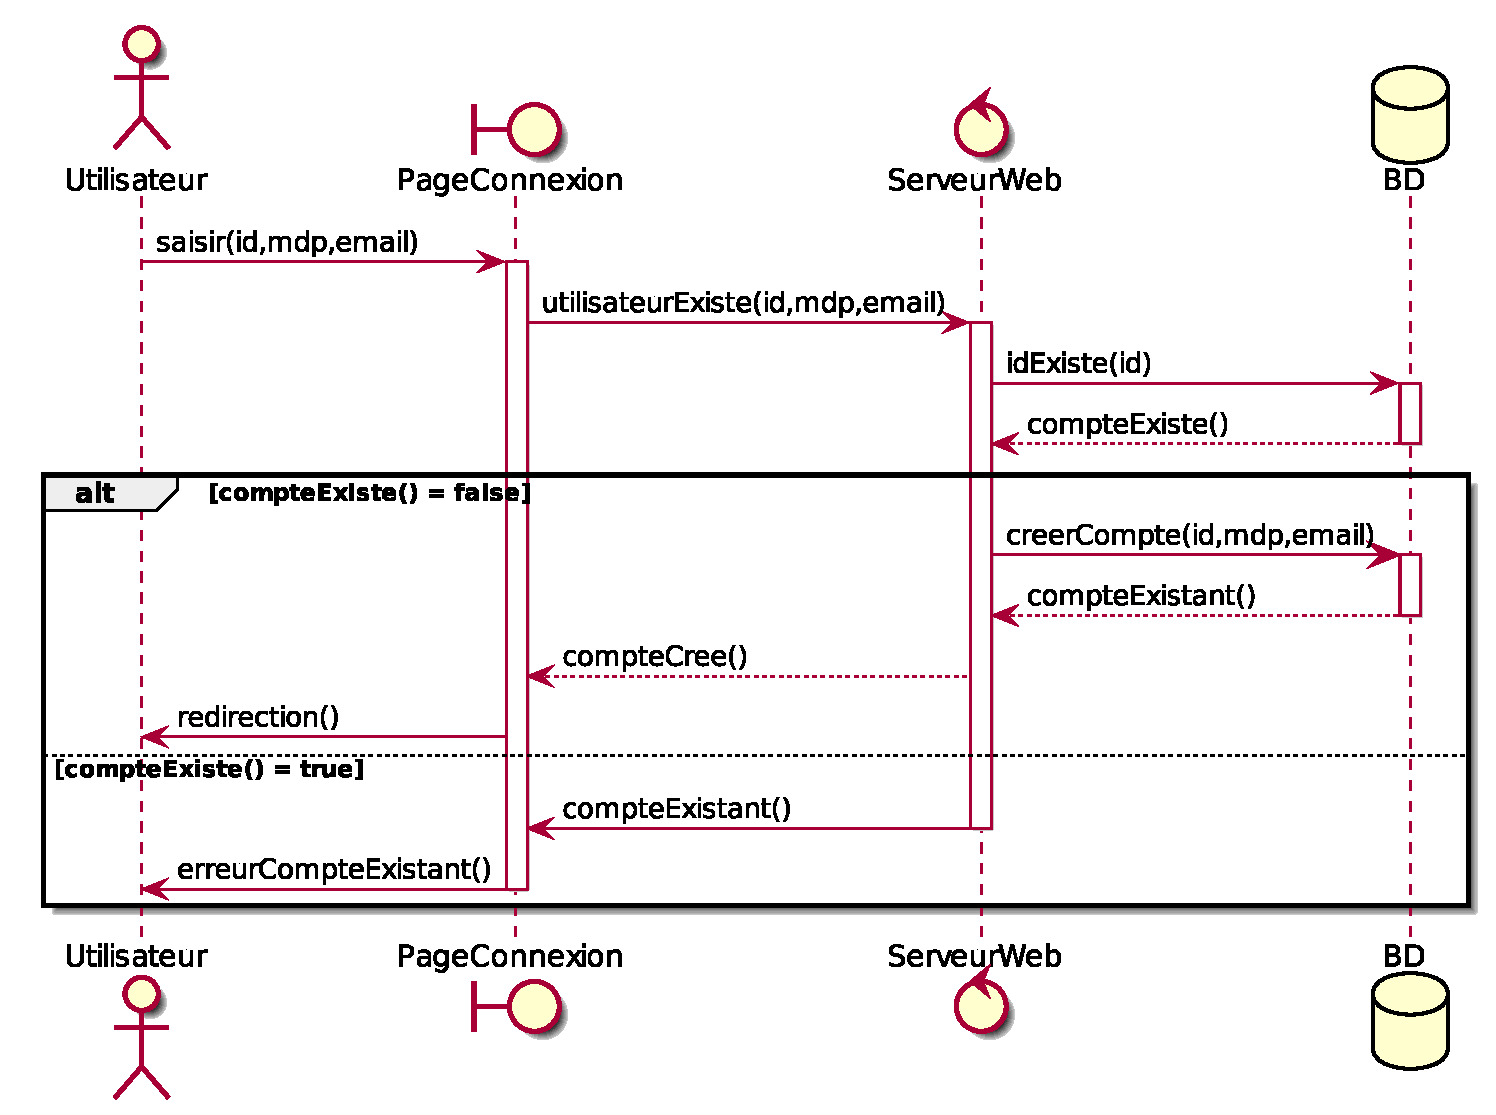
\includegraphics[width=15cm]{Images/DSEQ_CreationCompte} \\
\newpage
\subsubsection{Gestion d'un compte}
L'internaute peut procéder à la mise à jour de ses informations personnelles depuis la page de gestion du compte.\\
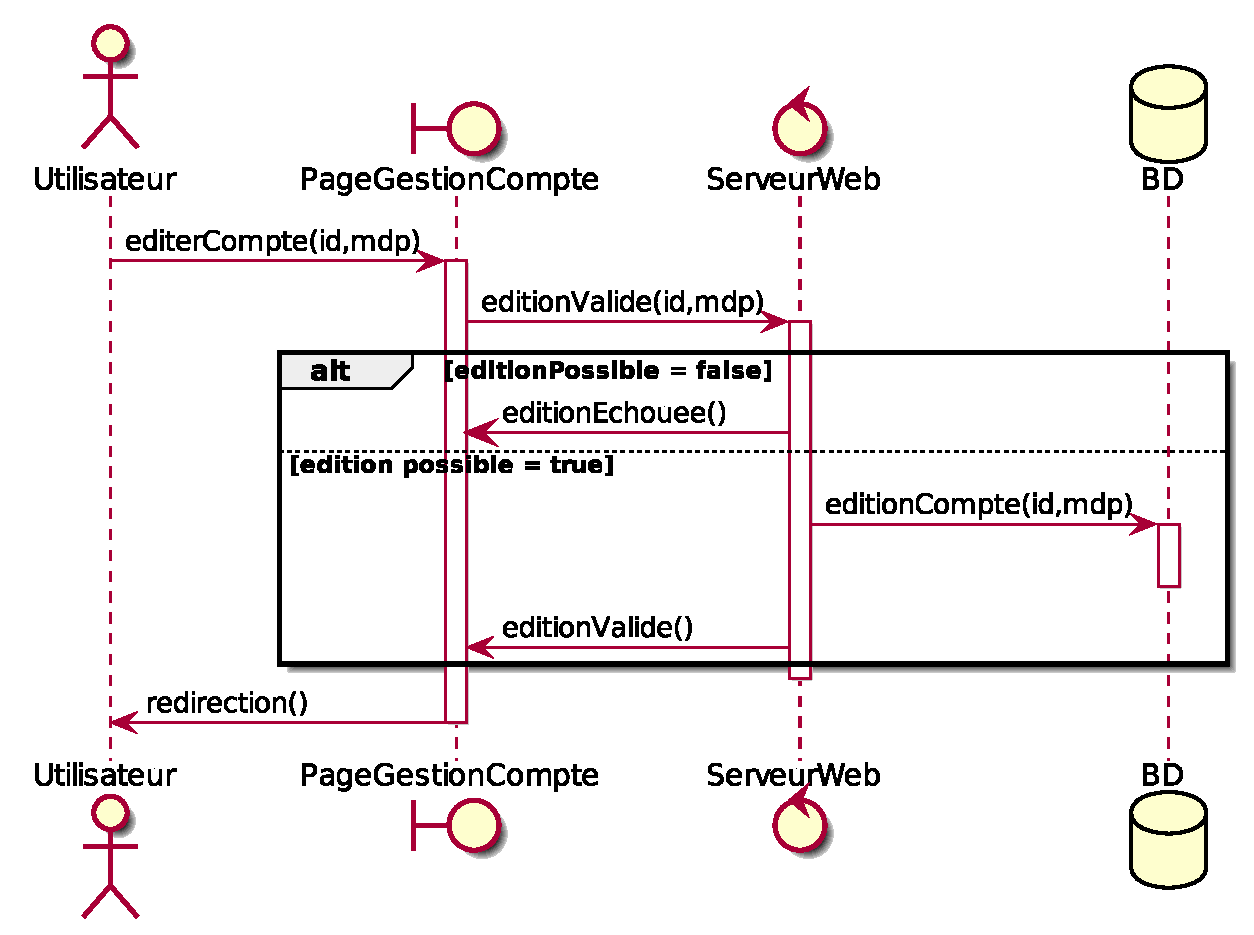
\includegraphics[width=17cm]{Images/DSEQ_GestionCompte} \\
\newpage
\subsubsection{Type de connexion}
Plusieurs type de connexion sont possibles : administrateur ou simple utilisateur \\
\includegraphics[width=17cm]{Images/DSEQ_TypeConnexion} \\
\newpage
\subsubsection{Recherche rapide ou avancée d'un objet}
Une fois sur le site, l'internaute souhaite trouver un objet à acheter selon ses critères. Pour cela, deux modes de recherche sont disponible, la recherche rapide selon une phrase entrée ou alors une recherche avancée selon le type, le prix et le lieu de vente de l'objet. \\
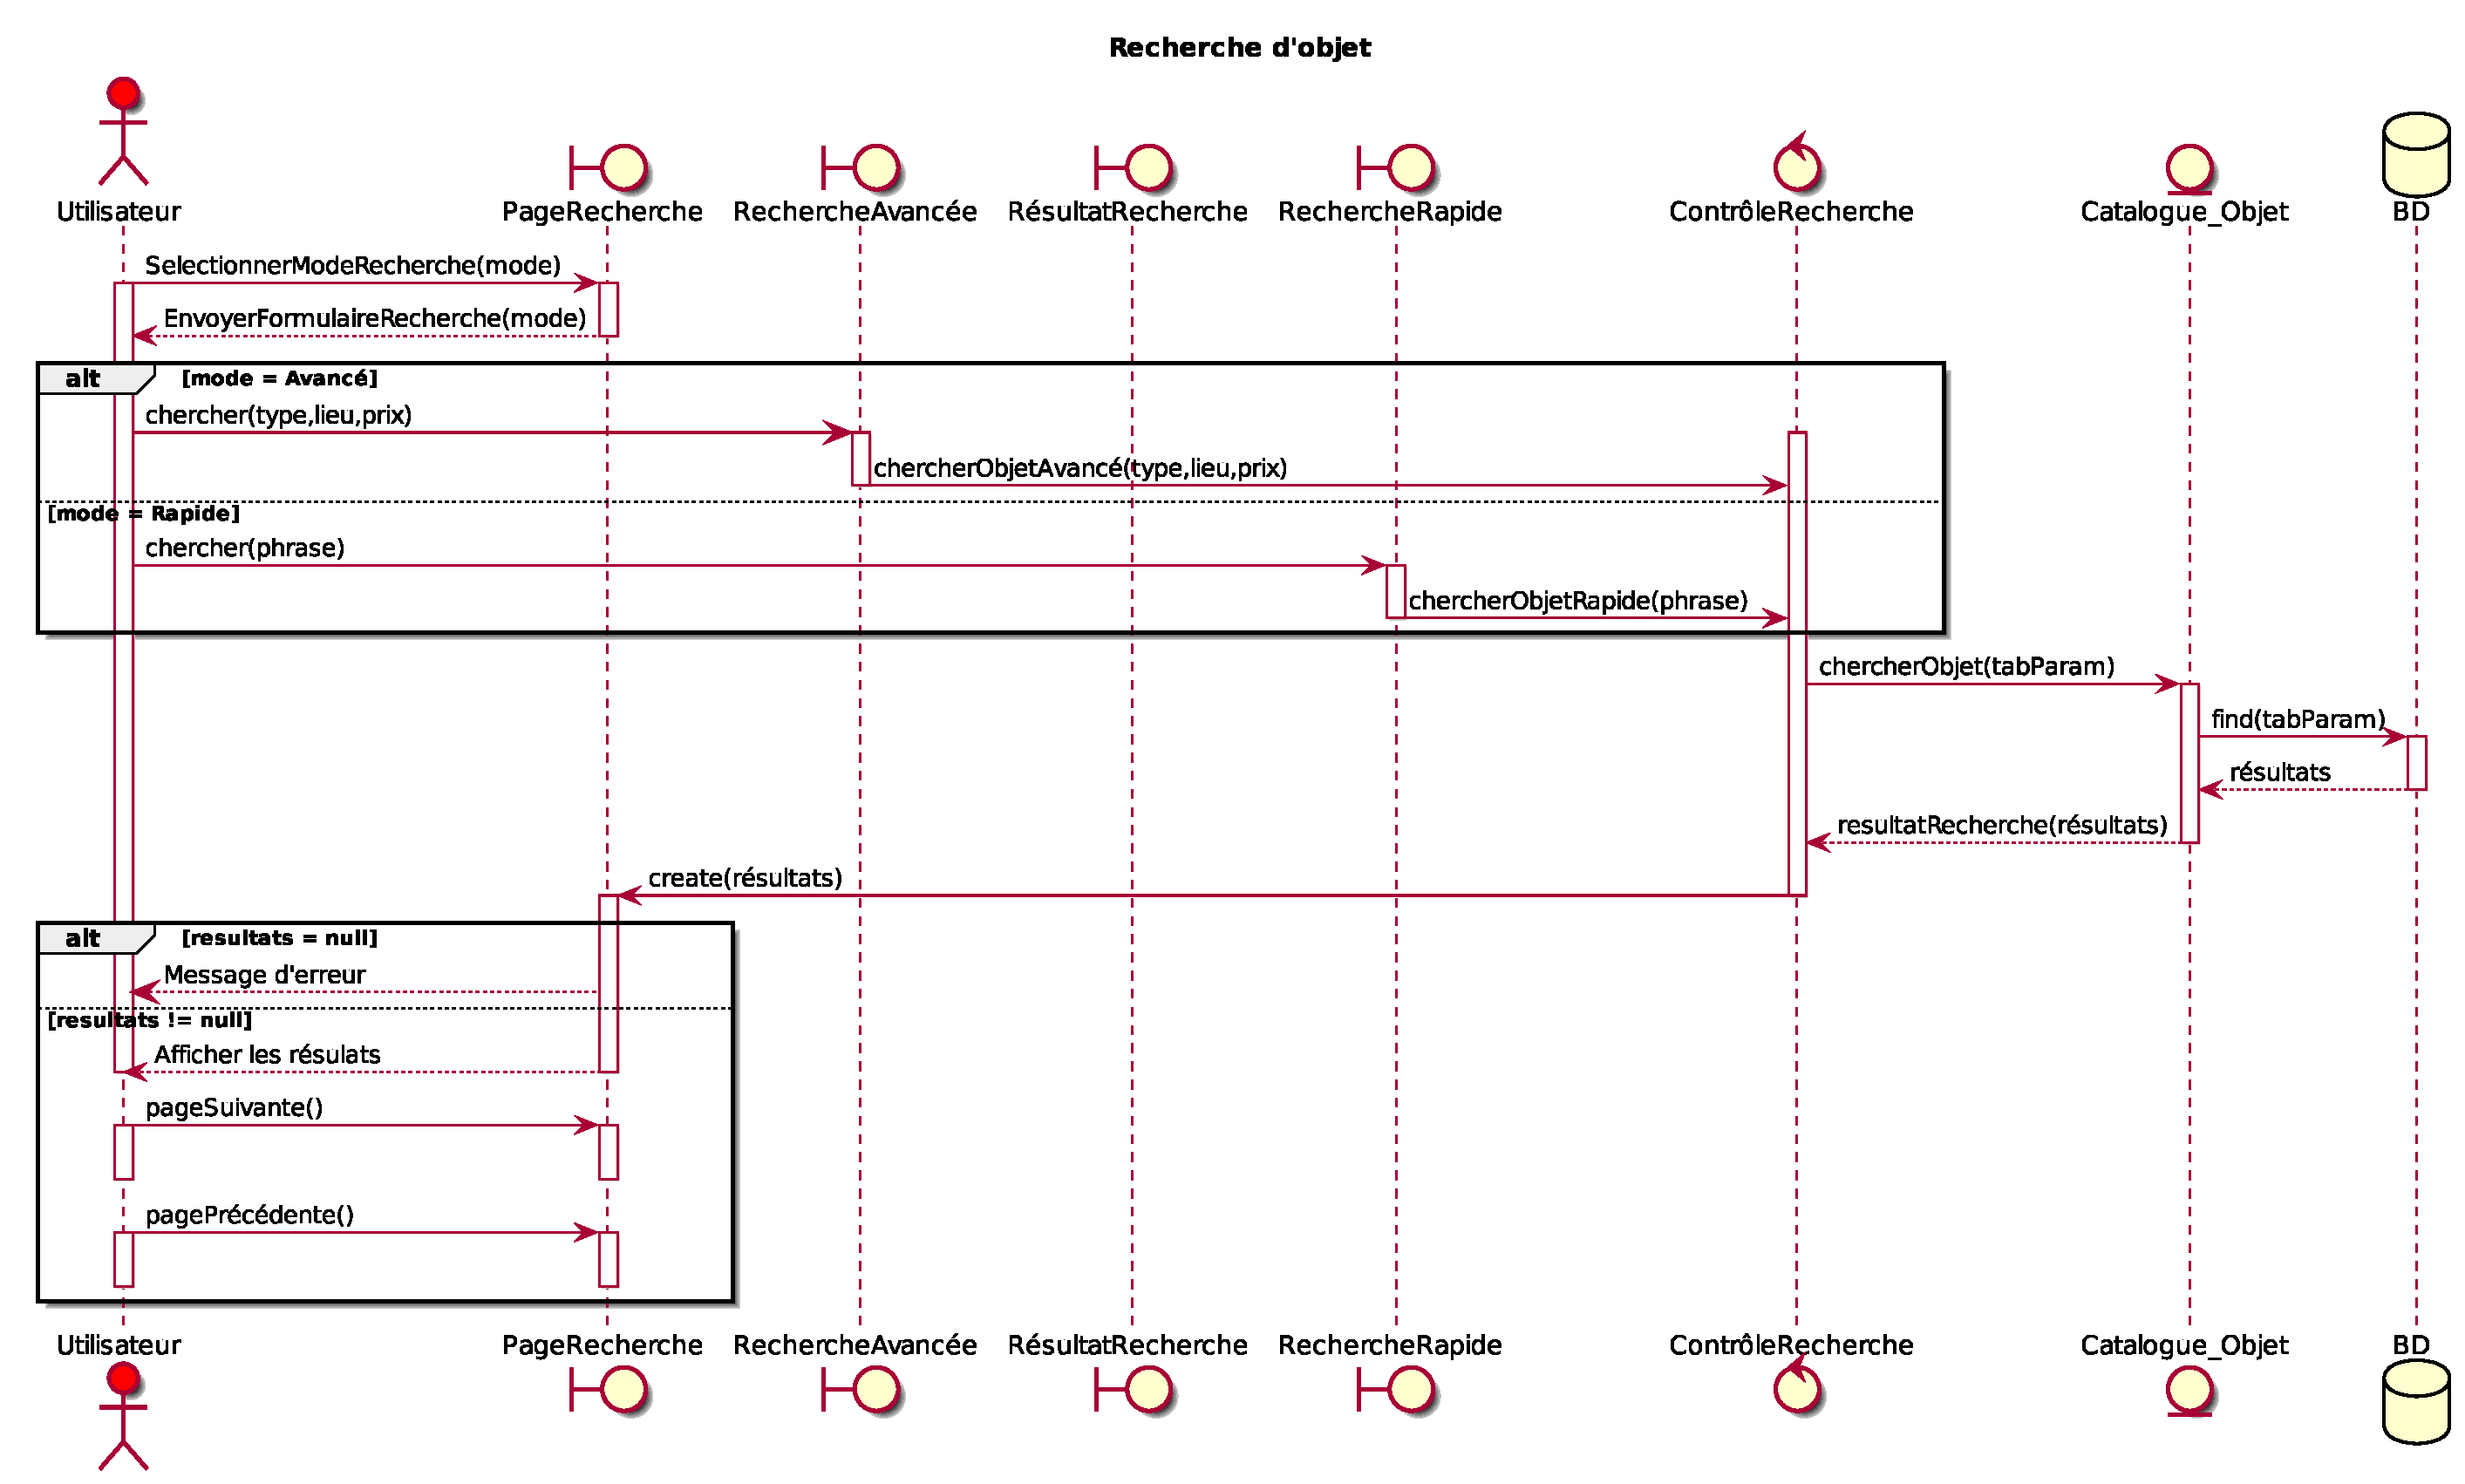
\includegraphics[width=17cm]{Images/DSEQ_Recherche} \\
\newpage
\subsubsection{Consultation d'un objet}
Lorsqu'une annonce intéressante est trouvée par l'internaute, il peut la consulter afin d'avoir des détails sur l'objet en vente tel que sa photo (facultative), son prix et sa description. \\
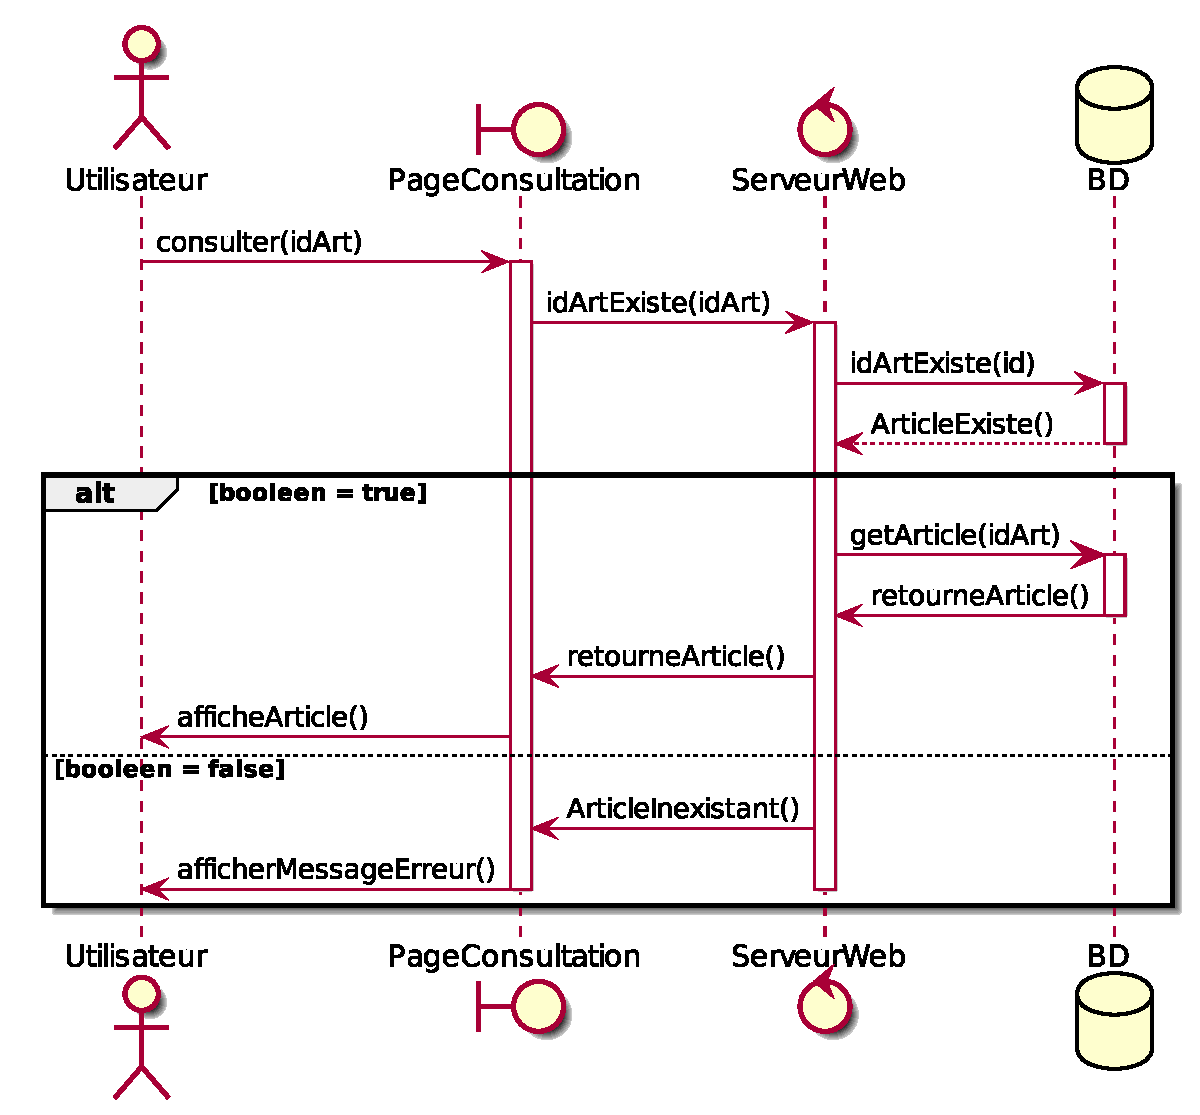
\includegraphics[width=17cm]{Images/DSEQ_Consultation} \\
\newpage
\subsubsection{Mise en vente}
L'internaute peut également mettre en vente un objet. Il doit renseigner les informations relatifs à l'objet pour que l'annonce puisse paraître. \\
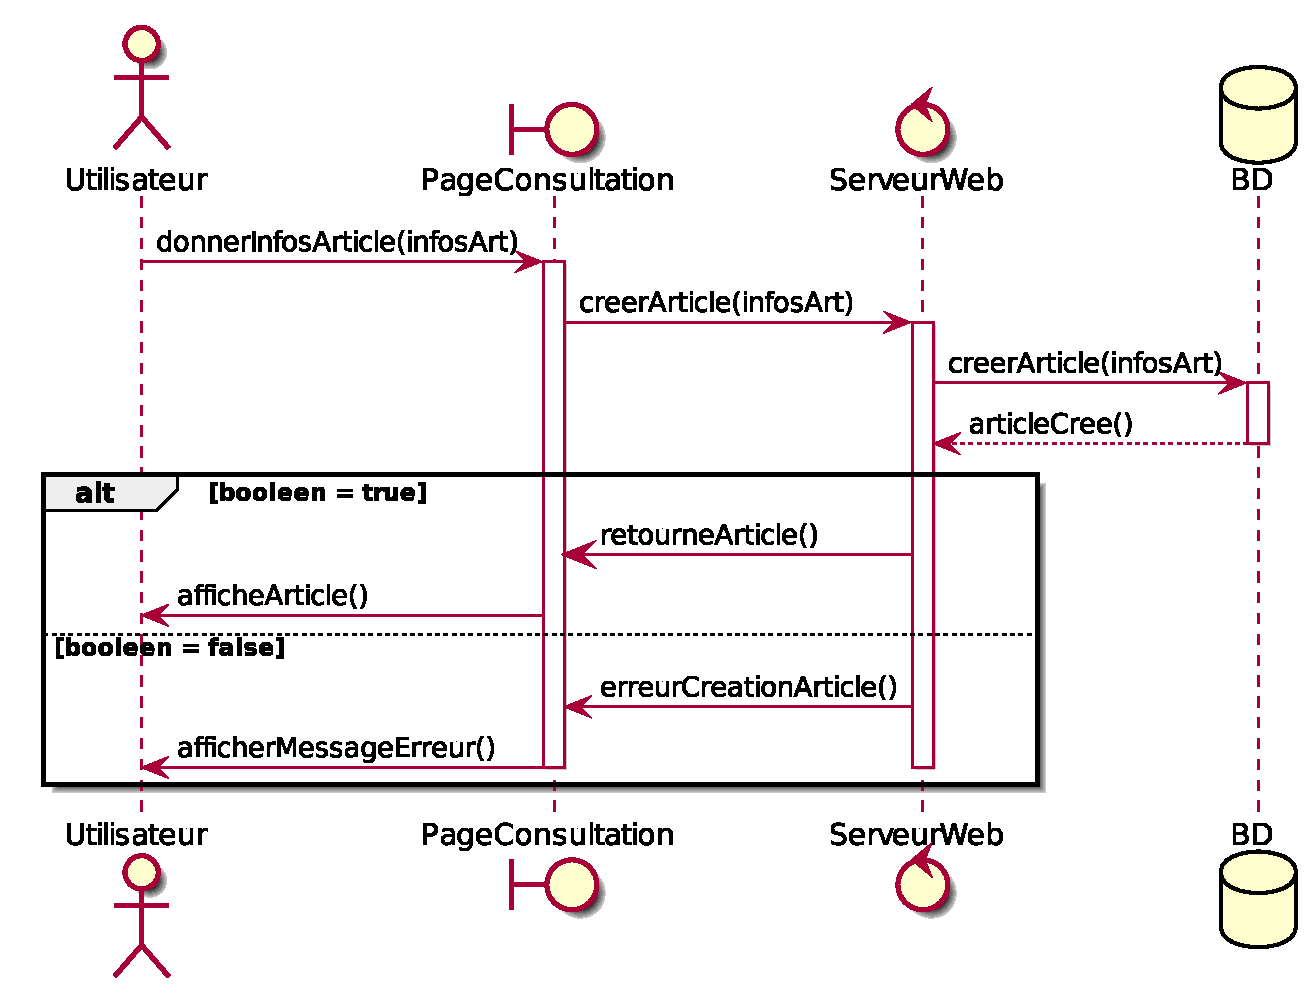
\includegraphics[width=17cm]{Images/DSEQ_MiseEnVente} \\
\newpage
\subsubsection{Panier}
L'internaute peut ajouter ou supprimer des articles de son panier en vue d'une commande. \\
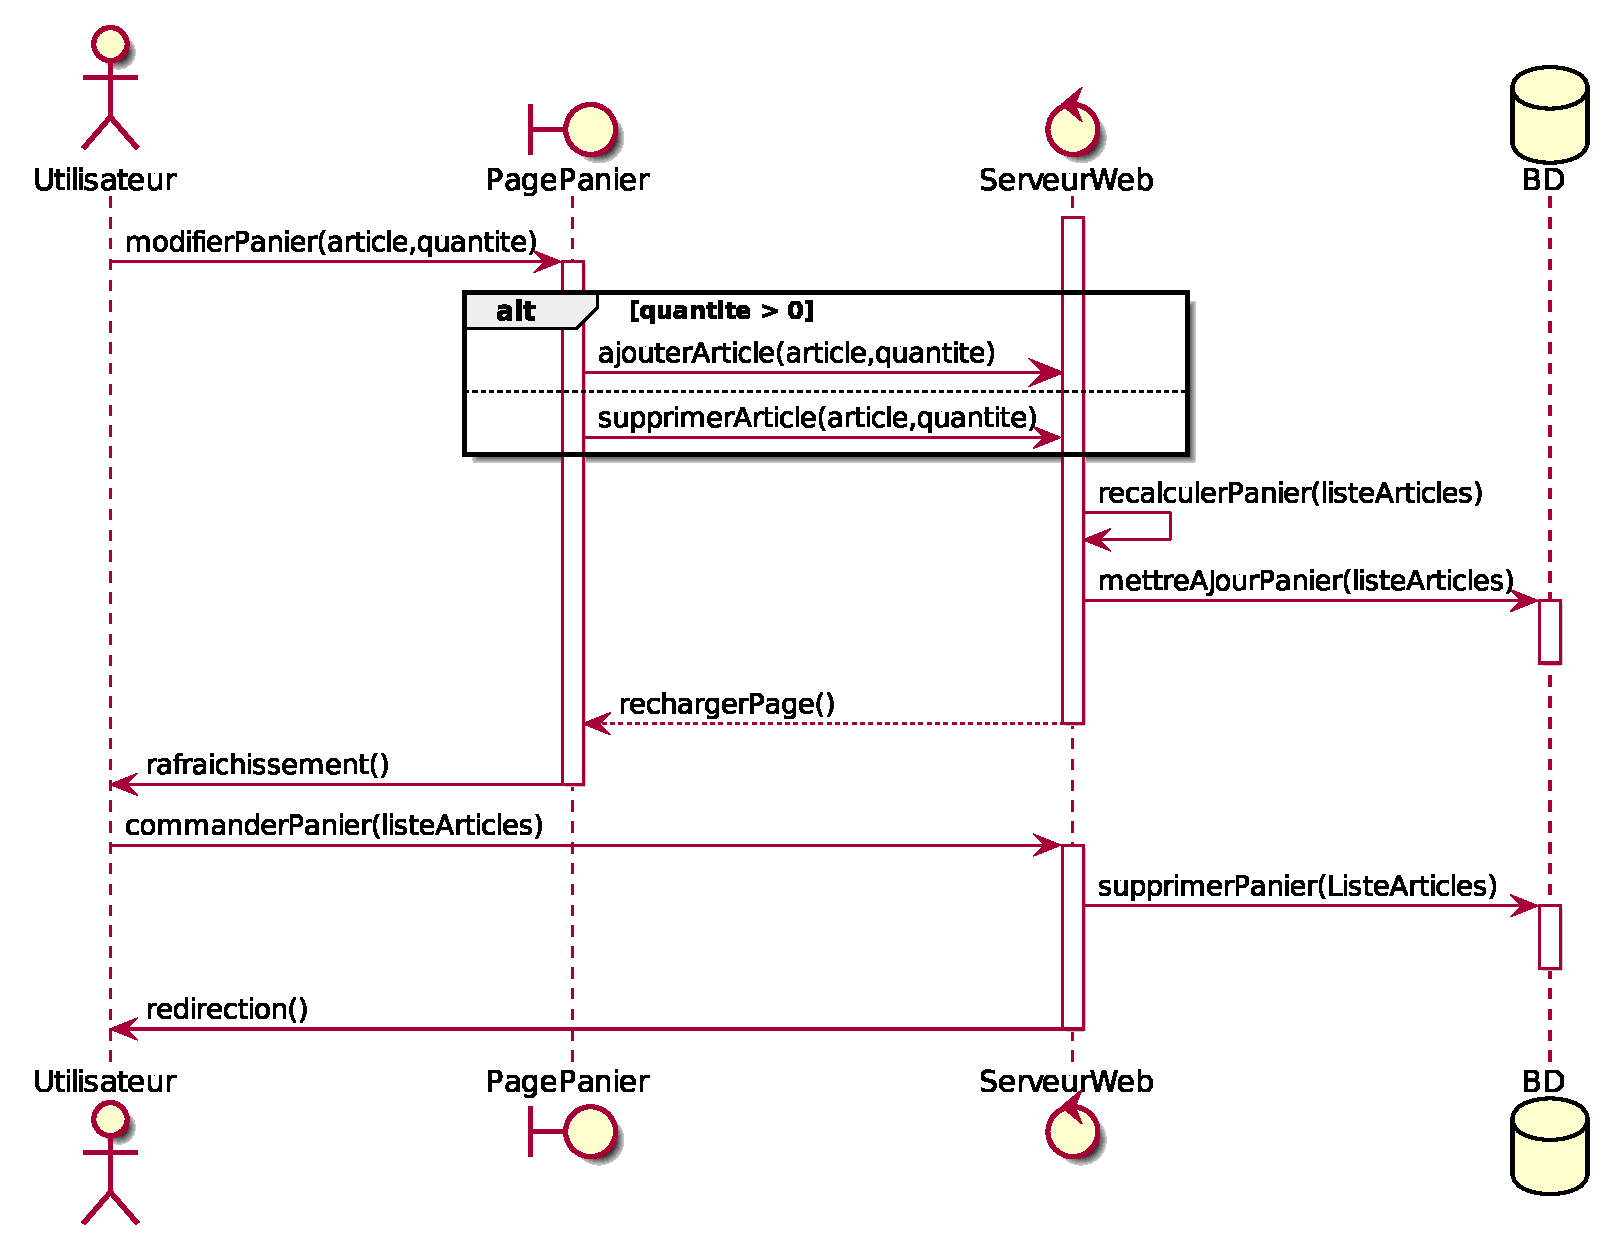
\includegraphics[width=17cm]{Images/DSEQ_Panier} \\
\newpage
\subsubsection{Paiement}
Lors de la mise en panier d'un ou plusieurs objets, l'internaute peut procéder au paiement en entrant ses coordonnées bancaires. \\
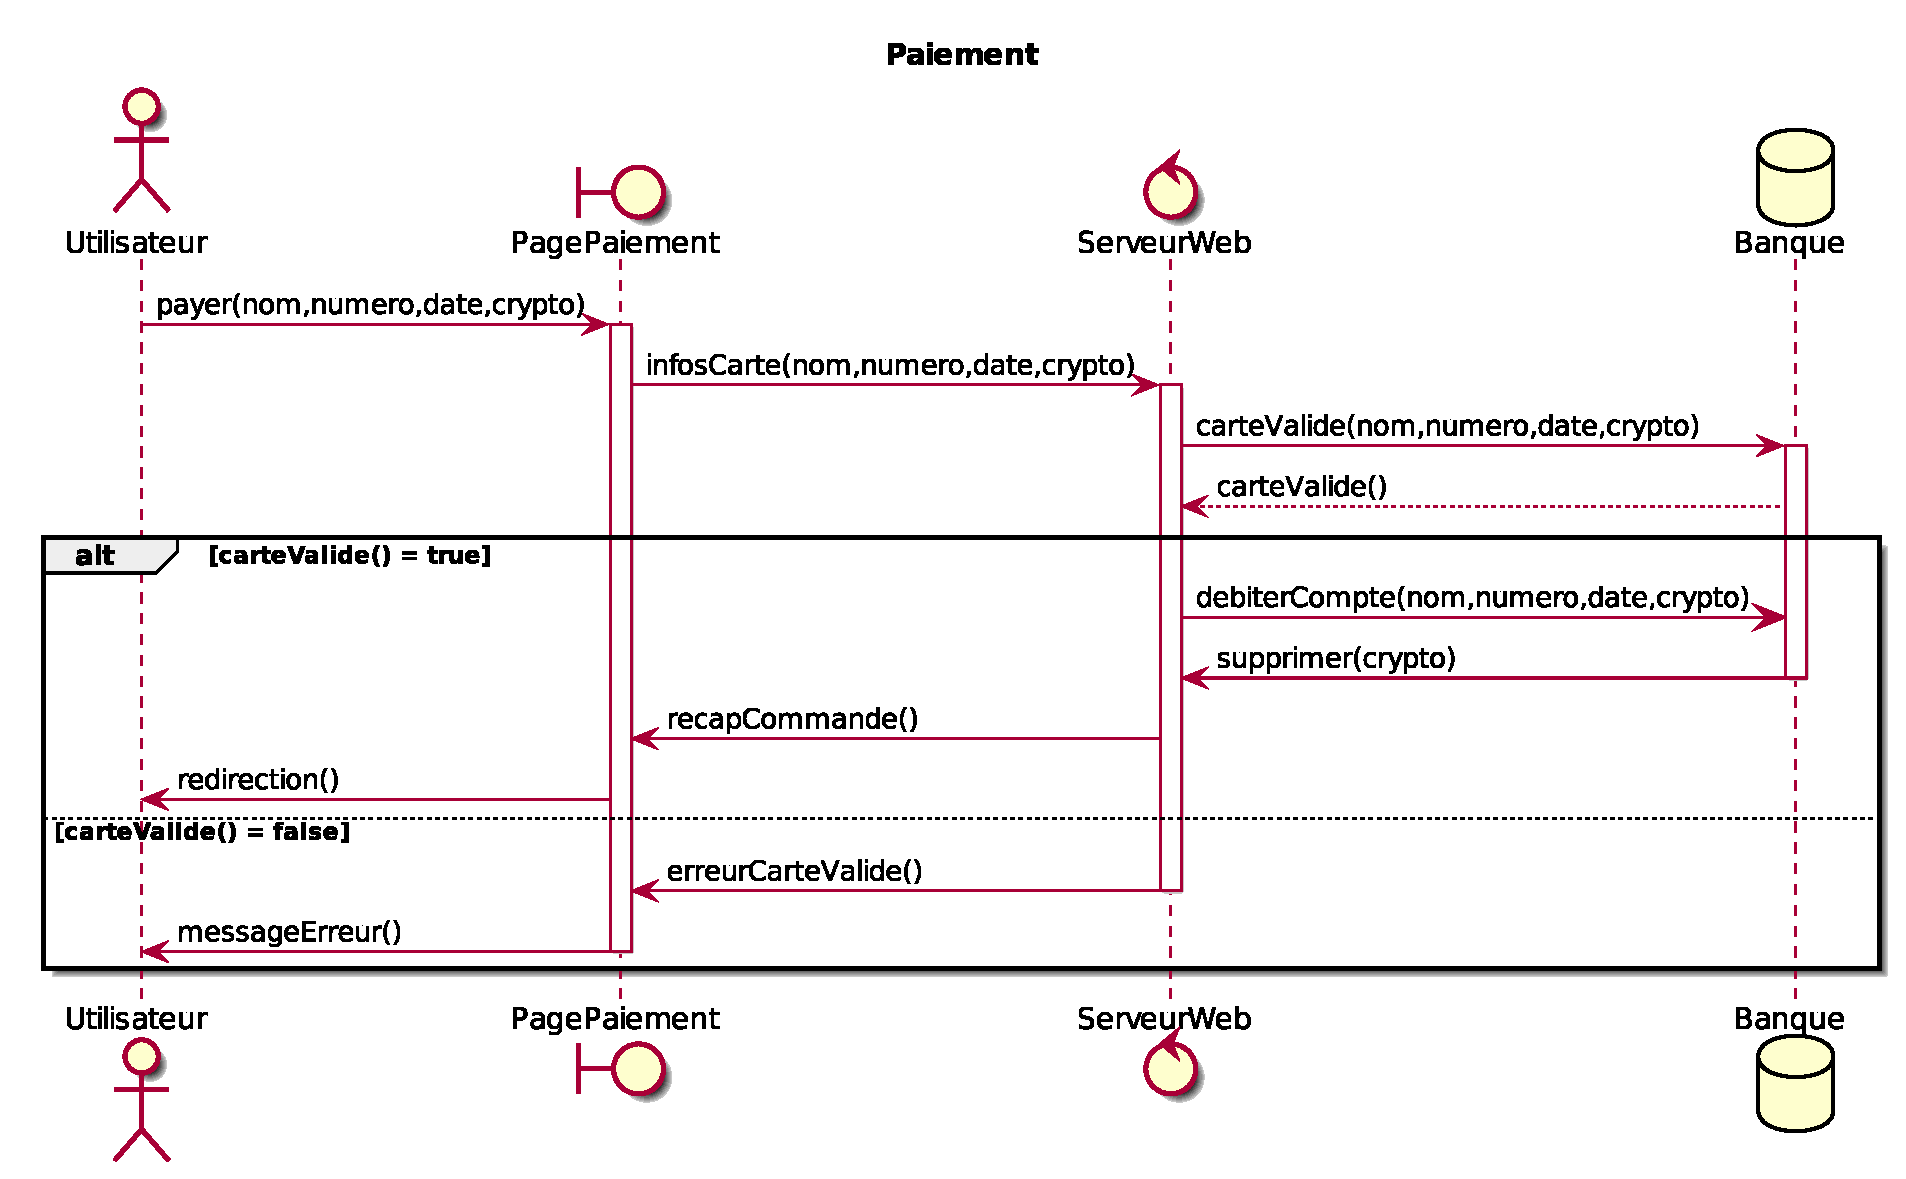
\includegraphics[width=17cm]{Images/DSEQ_Paiement} \\
\newpage
\subsubsection{Vote}
Lorsque la transaction est finalisée, l'internaute peut noter le vendeur. La note de celui-ci sera ainsi mise à jour. \\
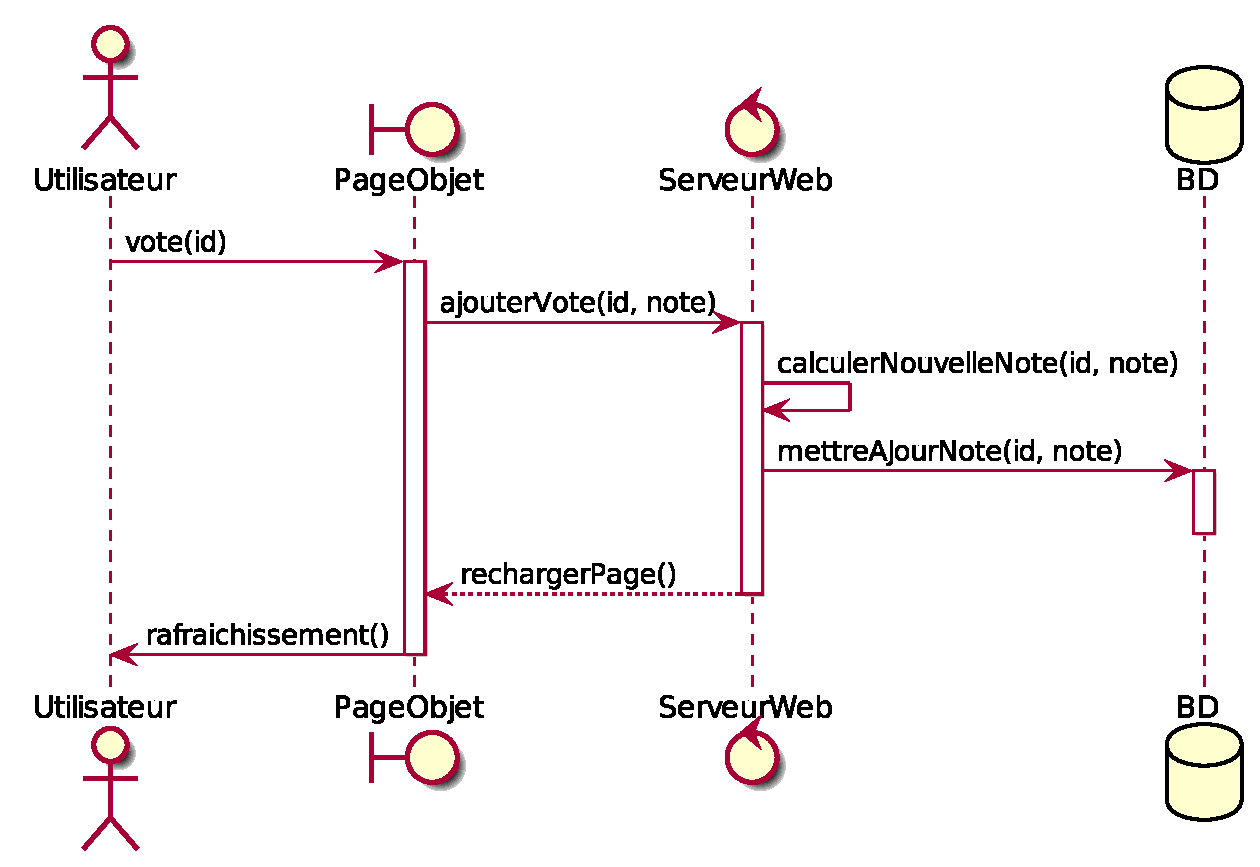
\includegraphics[width=17cm]{Images/DSEQ_Vote} \\
\newpage
\subsubsection{Messagerie}
Il est possible à l'internaute de demander des renseignements sur un objet mis en vente en envoyant un message au vendeur. Le contenu du message doit être validé au préalable par le modérateur. \\
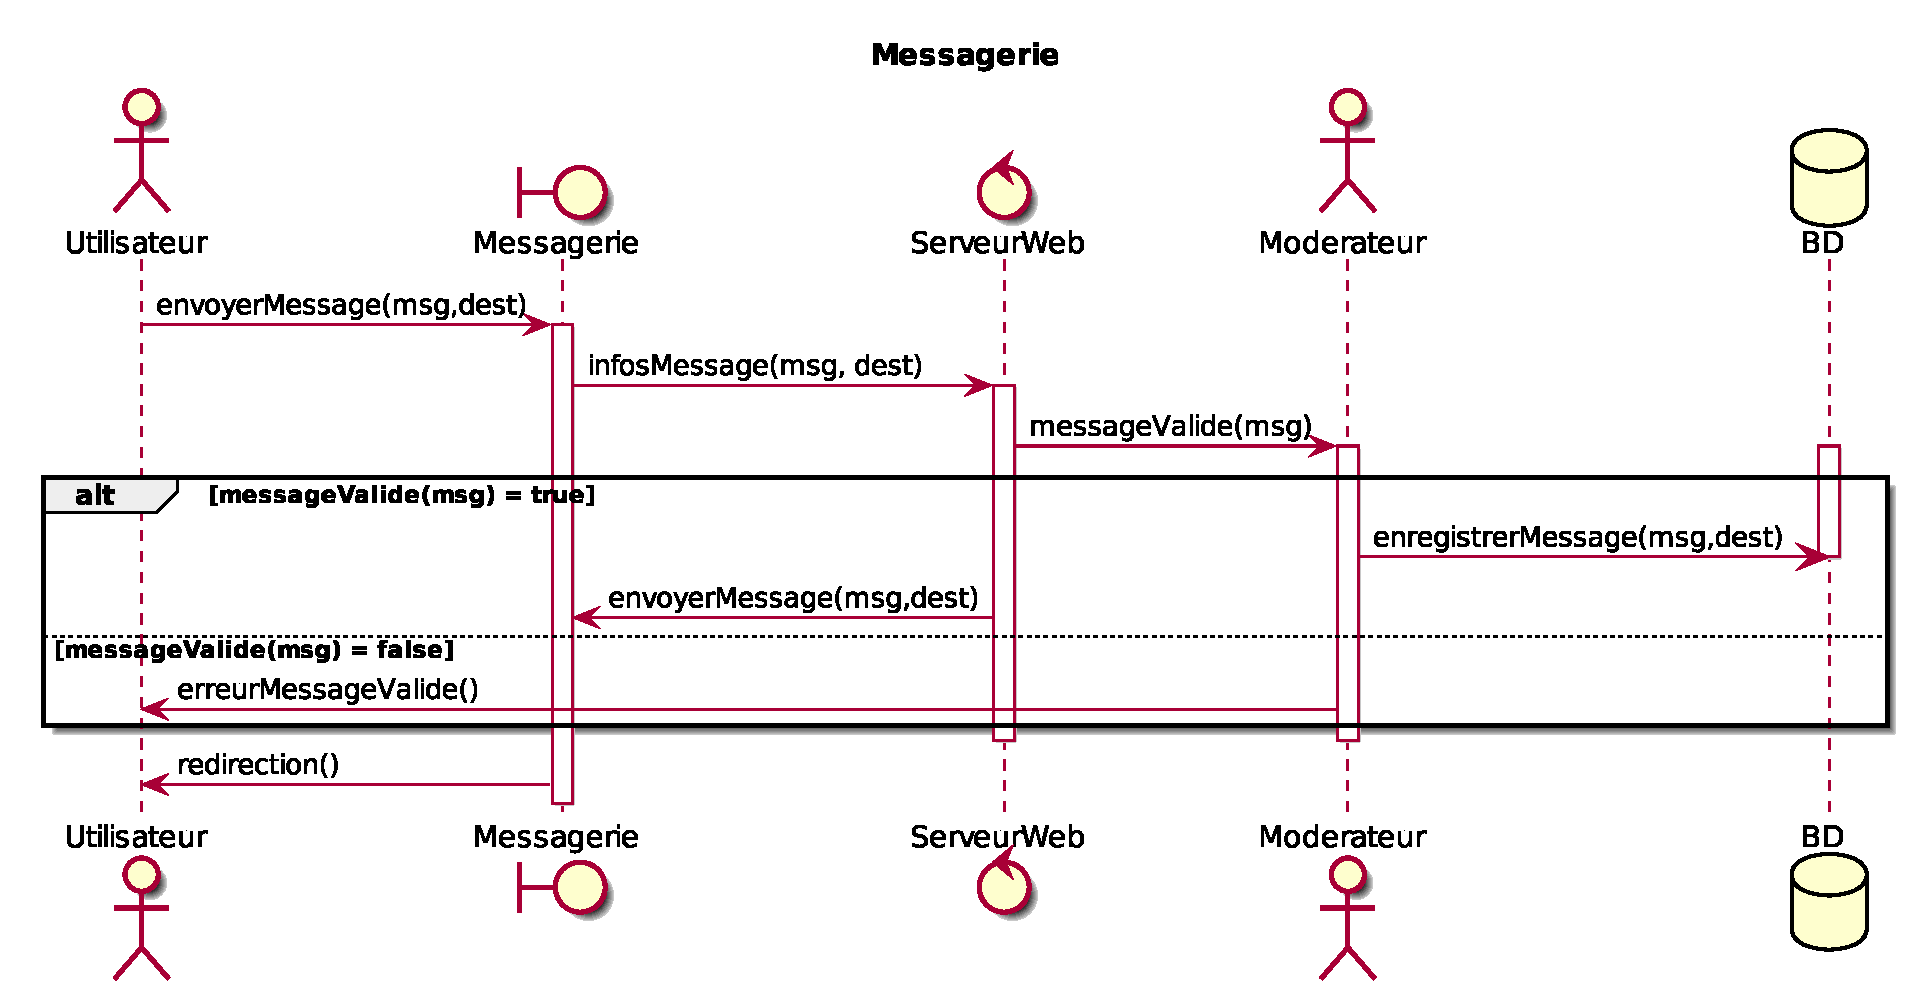
\includegraphics[width=17cm]{Images/DSEQ_Messagerie} \\
